%%%%%%%%%%%%%%%%%%%%%%%%%%%%%%%%%%%%%%%%%

%----------------------------------------------------------------------------------------
%       Paquetes y configuraciones
%----------------------------------------------------------------------------------------

\documentclass[11pt, a4paper]{article} % Font size
\usepackage[sfmath]{kpfonts}
\renewcommand*\familydefault{\sfdefault}

\usepackage{charter} % Use the Charter font for the document text
\usepackage[utf8]{inputenc}
\usepackage[T1]{fontenc}
\usepackage[spanish,es-nolayout,es-nodecimaldot,es-tabla]{babel}
\usepackage{amsmath}
\usepackage{amsfonts}
\usepackage{amssymb,amsthm}
\usepackage{enumerate}
\usepackage{enumitem}
\usepackage{parskip}
\usepackage{listings}
\usepackage{nicefrac}
\usepackage{framed, color}
\usepackage{graphicx}
\usepackage[left=2cm,right=2cm,top=2.5cm,bottom=2cm]{geometry}
\usepackage[colorlinks = true]{hyperref} 
\usepackage{wrapfig}
\usepackage[font={footnotesize,it}]{caption}

%
%       Configuración de Problema y Proposición
%
\definecolor{db}{RGB}{0,128,128}                % Color de pregunta y respuesta
\definecolor{dg}{RGB}{128,0,128}                % Color de proposiciones y teoremas
\definecolor{dh}{RGB}{128,128,0}                % Color de preguntas adicionales
\definecolor{da}{RGB}{0,102,153}                % Color de direcciones electrónicas
\newtheorem{teo}{Teorema}

\newtheoremstyle{dotlessP}{1em}{\topsep}{\color{db}}{}{\color{db}\bfseries}{}{ }{}
\theoremstyle{dotlessP}
\newtheorem*{prob}{Problema:}

\newtheoremstyle{dotlessS}{1em}{\topsep}{\color{dg}}{}{\color{dg}\bfseries}{}{ }{}
\theoremstyle{dotlessS}
\newtheorem*{prop}{Proposición:}


% Comandos
\newcommand{\R}{\mathbb{R}}
\newcommand{\dsum}{\displaystyle \sum}
\newcommand{\yds}{\qquad\text{y}\qquad}
\DeclareMathOperator{\Dom}{Dom}
\DeclareMathOperator{\Ran}{Ran}
\DeclareMathOperator{\inv}{inv}


% Revisa para posible uso: http://principiae.be/pdfs/TUG-X-004-slideshow.pdf
%---------------------------------------------------------------------------------------------
%       Recursos desarrollados en la Comunidad virtual – Tutoría en línea
%---------------------------------------------------------------------------------------------

% Tipo de documento
\newcommand{\tipodedocumeto}{Curso de preparación al examen Ser bachiller}

% Autor
\newcommand{\autor}{Fabricio}

% Editores
\newcommand{\editores}{Andrés Miniguano Trujillo y Juan Carlos Trujillo}

% Correos electrónicos
\newcommand{\email}{\href{mailto:refasabu@hotmail.com}{\color{da}refasabu@hotmail.com}}

\newcommand{\emaila}{\href{mailto:andres.miniguano@epn.edu.ec}{\color{da}andres.miniguano@epn.edu.ec}}

\newcommand{\emailb}{ y \href{mailto:jcto36@gmail.com}{\color{da}jcto36@gmail.com}}

% Fecha de creación de la pregunta
\newcommand{\creacion}{5 de abril de 2017}

% Fecha de publicación del recurso
\newcommand{\publicacion}{5 de abril de 2017}

% Título del recurso
\newcommand{\titulo}{Preguntas}


\usepackage{fancyhdr}
\pagestyle{fancy}
\renewcommand{\headrulewidth}{0pt}
\chead{\titulo}


\usepackage{lastpage}
\cfoot{\thepage\ de \pageref{LastPage}}


%----------------------------------------------------------------------------------------

\begin{document}\thispagestyle{empty}



%----------------------------------------------------------------------------------------
%       Contenidos
%--------------------------------------------------------------------------------------

\begin{enumerate}[label=\color{dg}\theenumi.]
        \setcounter{enumi}{30}
        \item {\color{db}
        El gráfico representa las posibles combinaciones de productos en relación con los costos de producción de \(x\) pantalones y \(y\) camisas. La función de costo está expresada por C=\(12x+6y\). Determine la cantidad de pantalones y camisas que reducen el costo de producción.}
        
        
        Necesitas la cantidad de pantalones y camisas que representen un costo de producción menor, por lo tanto debes remplazar la cantidad de cada literal en la ecuación de costo de producción y elejir la que represente menor costo.
        
        Al remplazar en las ecuaciones tienes que al producir \(1\) pantalón y \(3\) camisas genera un costo menor de producción.
        
        {\color{dh} \((1)\) \(1\) pantalón y \(3\) camisas
        
        \((2)\) \(1\) pantalón y \(12\) camisas
        
        \((3)\) \(3\) pantalónes y \(1\) camisa
        
        \((4)\) \(5\) pantalónes y \(1\) camisa}
        

        
       \[ C= 12x + 6y\]
         \[ C= 12(1) + 6(3)\]
         \[ C= 12 + 18\]
         \[ C=30\]
        
 {\color{dh}La respuesta correcta es la 1.}

%---------------------------------------------------------------------------
		\item {\color{db}
        Se han tabulado las notas de \(4\) grupos de un colegio en 5 materias distintas. Con base en la tabla }
        
        
        \begin{table}[htbp]
		\centering
		\label{my-label}
	\begin{tabular}{|c|c|c|c|c|}
		\hline
		\textbf{       } & \textbf{Grupo 1} & 					\textbf{Grupo 2} & \textbf{Grupo 3} & \textbf{Grupo 4}
        
         \\ \hline
		Materia 1                & 5,00          & 10,00    
        &10,00  &8,00\\ \hline
		Materia 2                 & 6,00           & 8,00 
        &9,00  &9,00  \\ \hline
		Materia 3                 & 5,00       & 10,00    
        &10,00  &9,00\\ 		\hline
		Materia 4                 & 6,00        & 4,00 
        &8,00  &9,00\\ 		\hline
		Materia 5                  & 5,00           & 5,00 
        &9,00  &8,00\\ 		\hline
		 Promedio                 & 5,40        & 7,40    
         &9,20  &8,80 \\ 		\hline
         Desviación estándar      & 0,49         &2,50
         &0,75  &0,40
        
        \\ 		\hline
      
        
        \end{tabular}
	\end{table}
        
         {\color{dh} \((1)\) grupo \(1\)
        
        \((2)\) grupo \(2\) 
        
        \((3)\) grupo \(3\) 
        
        \((4)\) grupo \(4\) }
        
        
         La desviación estándar mide cuan extendido es el rango de los datos en torno a la media y es una medida directa de dispersión, en el caso de los datos de la tabla el grupo con menor desviación estándar es el que tiene menos dispersas sus calificaciones, este grupo es el \(4\) con una desviación estándar de \(0,40\) 
        

		{\color {dh}La respuesta correcta es la 4.}
  %-------------------------------------------------------------------------------      
        
        \item{\color{db}
    Un grupo de arqueólogos ha delimitado una área triangular de \(150m^2\) 
    para sus estudios sobre una civilización antigua. Determine , en metros, la medida de la base a delimitar si se establece que la misma tiene que ser el cuádruplo de la altura.}
    
     {\color{dh} \((1)\) \(5\sqrt[2]{3} m\)
        
        \((2)\) \(10\sqrt[2]{3} m\)
        
        \((3)\)  \(15\sqrt[2]{3} m\) 
        
        \((4)\) \(20\sqrt[2]{3} m\) }
        
        La base que tienes es trangular el valor es de \(150m^2\).
        
        La base de un triángulo es:
   
   \begin{center}
     \(A\)= \( \frac{base*altura}{2}\)
       \end{center}
       
        
       La medida de la base a delimitar es el cuádruplo de la altura:
       \begin{center}
       
       \(b=4h\) 
      
      \(h\)=\(\frac{b}{4}\)
      \end{center}
       
       Reemplaza los valores en la ecuación del área
       
       
       \(A\)= \( \frac{b*h}{2}\)
      
    \(150m^2\)= \( \frac{b*b}{8}\)
    
           \(150m^2*8\)  = \( b^2\)
           
           \(1200m^2\)=\(b^2\)
           
         \(\sqrt[2]{1200m^2}\)=\(\sqrt[2]{b^2}\)
         
         \(b\)=\(20\sqrt[2]{3} m\)
           
           
       
        {\color{dh}La respuesta correcta es la 4.}
%---------------------------------------------------------------------------------
		\item{\color{db}
        Un banco ofrece un plan de inversión en el cual las ganancias estan definidas por la ecuación 
        
        \[ C(t)= Co.K^{(t-1)} ; t>0, donde:\]
        
        \(Co\) es la inversión inicial.
        
      La tasa de rendimiento \(k\)=\(\frac{5}{3}\).
      
      El tiempo \(t\) esta dado en meses.
        
       Si una persona decide invertir USD \(21879\). ¿cuánto dinero, en dólares, habrá ganado dentro de\(4\) meses?}
       
        {\color{dh} \((1)\) \(3375\)
        
        \((2)\) \(5625\)
        
        \((3)\)  \(10125\) 
        
        \((4)\) \(16875\) }
       
       
       Tienes la inversión inicial de USD \(21879\)
       
       El tiempo \(t\)= \(4 meses \)
       
       La tasa de rendimiento \(k\)=\(\frac{5}{3}\).
       
     Reemplaza los datos dados,en la ecuación  \(C(t)= Co.K^{(t-1)}\)
     
     \(C(t)=21879*\frac{5}{3}^{ (4-1)}\)
     
     \(C(t)=21879*\frac{125}{27}\)
     
      \(C(t)=10125\)
    
       {\color{dh}La respuesta correcta es la 3}
         
%-----------------------------------------------------------------------------

        \item{\color{db}
        Hace \(3\) años la edad de Lourdes era el cuádruplo que la de su hijo y después de \(7\) años será el doble. Actualmente, ¿ cuál es la edad de Lourdes y de su hijo? }
        
         {\color{dh} \((1)\)  \(20\) y \(5\)
        
        \((2)\) \(23\) y \(8\)
        
        \((3)\)  \(29\) y \(11\) 
        
        \((4)\) \(33\) y \(6\) }
        
         Primeramente, llama \(x\) a la edad de Lourdes y a la edad de su hijo \(y\),luego tienes que hace \(3\) años la edad de Lourdes era el cuádruplo que la de su hijol \(x-3\)=\(4(y-3)\) y después de \(7\) años es el doble \(x+7\)=\(2(y+7)\). Finalmente, Despejas \(x\) en ambas ecuaciones 
         
         primera ecuación
        
        \(x-3\)=\(4(y-3)\)
         
         \(x-3\)=\(4y-12\)
         
         \(x\)=\(4y-9\)
         
         Segunda ecuación
         
         \(x+7\)=\(2(y+7)\)
         
         \(x+7\)=\(2y+4\)
         
         \(x\)=\(2y+7\)
         
         Una vez que despejes iguala la primera y segunda ecuación 
         
         \(4y-9\)=\(2y+7\)
         
        \(2y\)=\(16\)
        \(y\)=\(8\)
        
        reemplaza \(y\) en cualquiera de las dos ecuaciones 
        
        \(x\)=\(4y-9\)
        
        \(x\)=\(4*(8)-9\) 
        
         \(x\)=\(23\)
        
        
     
		{\color{dh}La respuesta correcta es la 2.}
        


\end{enumerate}



\begin{enumerate}[label=\color{dg}\theenumi.]
        \setcounter{enumi}{153}
        \item {\color{db} Seleccione la imagen que continúa la secuencia}
        
        Primeramente, se ve que la línea gira en dirección a las manecillas del reloj, luego en cada recuadro  la línea va cambiando. Finalmente la imagen que continúa la secuencia es la \(2\) ya que esta regresa a su forma original.
        
        
        
        
         {\color{dh}La respuesta correcta es la 2}
 %------------------------------------------------------------------------------
 
 \item{\color{db}Identifique la figura que completa la secuencia} 
 
 Primeramente, se ve que la figura gira en sentido contrario a las manecillas del reloj, luego de igual manera se ve que las figuras cambian de posición manteniendo el orden de los graficos que estan dentro. Finalmente la figura que corresponde es la \(2\) ya que esta regresa a su forma original.
 
 
 
 
 
 {\color{dh}La respuesta correcta es la 2}
 %----------------------------------------------------------------------------
 
 \item{\color{db}Seleccione la imagen que continúa la matriz}
 
 Toma en cuenta que el cuadrado pequeño siempre va dentro del cuadrado más grande , luego se ve que el gráfico del círculo con tres líneas esta bajando en cada secuencia de igual manera la parte sombreada dentro del semiovalo va cambiando de posición. Finalmente al cambiar de posición la parte sombreada dentro el semiovalo se ve que este va de medio-derecha-izquierda en donde el resultado es el segundo.
 
 {\color{dh}La respuesta correcta es la 2}
%--------------------------------------------------------------------------------

\item{\color{db}Identifique la vista que pertenece a la gráfica}

\begin{center}

\includegraphics[scale=1]{157_1}
\end{center}

  {\color{dh}
\(1\) 
\includegraphics[scale=0.5]{15711}

\(2\)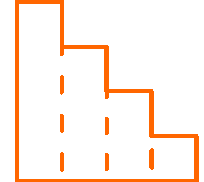
\includegraphics[scale=0.5]{1571}

\(3\)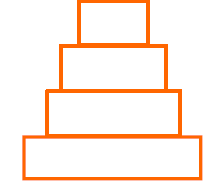
\includegraphics[scale=0.5]{1573}

\(4\) 
\includegraphics[scale=0.5]{1574} }

La respuesta correcta de la vista es la tercera 

{\color{dh}La respuesta correcta es la 3}

%--------------------------------------------------------------------------------

\item{\color{db}Identifique la figura que reemplaza a la incognita}

Primero, toma en cuenta que los circulos se mantienen en cada \(2\) secuencias, luego aumenta un círculo adicional, además la posición correcta en que aumenta es desde el vértice inferior hacia los demás vértices. Finalmnete de igual manera los lados del cuadrado va aumentando \(1\) cada \(2\) secuencias al igual que las estrellas.

{\color{dh}La respuesta correcta es la 1} 

%--------------------------------------------------------------------------------
  \item{\color{db}¿ Qué figura reemplaza a la incógnita ?}
  
   Primero, toma en cuenta que en cada secuencia va aumentando un gráfico dentro del círculo, luego el gráfico de color negro dentro del círculo cambia de posición en dirección a las manecillas del reloj. Finalmente la figura reemplaza a la incógnita es la \(2\).
  
 {\color{dh}La respuesta correcta es la 2}
%-------------------------------------------------------------------------------
  \item{\color{db}Complete la analogía}
        
        En la analogía se ve que la figura que esta dentro la primera imagen viene a estar fuera en la segunda imagen y viceversa,además toma en cuenta que tanto en la primera imagen y segunda imagen la combinación esta dada por figuras del mismo tipo siendo así la respuesta es la \(3\).
        
        {\color{dh}La respuesta correcta es la 3}
        
        
        \end{enumerate}
        















%----------------------------------------------------------------------------------------


\end{document}
       